% this template is an adaption of:
% https://www.overleaf.com/latex/templates/template-for-theoretische-informatik-uni-tubingen/xwsycshfkjtf


% change for each exercise
\newcommand{\NUMBER}{1}
\newcommand{\EXERCISES}{4}

% only once
\newcommand{\COURSE}{Introduction to Neural Networks, Summer Semester 2025}
\newcommand{\STUDENTA}{Finn Fassbender}
\newcommand{\STUDENTB}{Ahmet Alperen Güngör}


% keep as is --------------------------------------------------------
\documentclass[a4paper]{scrartcl}
\usepackage[utf8]{inputenc}
\usepackage[english]{babel}
\usepackage{amsmath}
\usepackage{amssymb}
\usepackage{fancyhdr}
\usepackage{graphicx}
\usepackage{lastpage}
\usepackage{listings}
\usepackage{tikz}
\usepackage{pdflscape}
\usepackage{subfigure}
\usepackage{float}
\usepackage{polynom}
\usepackage{hyperref}
\usepackage{tabularx}
\usepackage{forloop}
\usepackage{geometry}
\usepackage{listings}
\usepackage{fancybox}
\usepackage{tikz}
\usepackage{algpseudocode,algorithm,algorithmicx}
\usepackage{enumitem}
\usepackage{physics}
\renewcommand*{\arraystretch}{1.2}

\input kvmacros
\geometry{a4paper,left=3cm, right=3cm, top=3cm, bottom=3cm}

% headline
\def\header#1{
	\begin{center}
		{\Large Assignment Sheet #1}
	\end{center}
}

% point table
\newcounter{punktelistectr}
\newcounter{punkte}
\newcommand{\punkteliste}[2]{%
	\setcounter{punkte}{#2}%
	\addtocounter{punkte}{-#1}%
	\stepcounter{punkte}%<-- also punkte = m-n+1 = Anzahl Spalten[1]
	\begin{center}%
		\begin{tabularx}{\linewidth}[]{@{}*{\thepunkte}{>{\centering\arraybackslash} X|}@{}>{\centering\arraybackslash}X}
			\forloop{punktelistectr}{#1}{\value{punktelistectr} < #2 } %
			{%
				\thepunktelistectr &
			}
			#2 &  $\Sigma$ \\
			\hline
			\forloop{punktelistectr}{#1}{\value{punktelistectr} < #2 } %
			{%
				&
			} &\\
			\forloop{punktelistectr}{#1}{\value{punktelistectr} < #2 } %
			{%
				&
			} &\\
		\end{tabularx}
	\end{center}
}

% header / footer
\pagestyle {fancy}
\fancyhead[L]{\COURSE}
\fancyhead[C]{}
\fancyhead[R]{\today}

\fancyfoot[L]{}
\fancyfoot[C]{}
\fancyfoot[R]{Page \thepage /\pageref*{LastPage}}

\begin{document}
	
% don't change
\begin{tabularx}{\linewidth}{m{0.2 \linewidth}X}
	\begin{minipage}{\linewidth}
		\STUDENTA\\
		\STUDENTB
	\end{minipage} & \begin{minipage}{\linewidth}
		\punkteliste{1}{\EXERCISES}
	\end{minipage}\\
\end{tabularx}

\header{Nr. \NUMBER}
% -------------------------------------------------------------------

% your solution
% \begin{enumerate}[label=(\alph*)]


\section*{Question 1: Logistic Regression --- Theory}
\begin{enumerate}[label=(\alph*)]
	\item The likelihood is the probability that a distribution will produce a certain dataset or point of data. Find an expression for the likelihood of a single data point i.e. $P(y = y^{(i)} \mid x^{(i)}, \theta)$ and the likelihood of the whole dataset i.e. $P(y \mid X, \theta) = \prod_i P(y = y^{(i)} \mid x^{(i)}, \theta)$. This expression should match with the one in part (b) when you take the logarithm. \\
		\begin{align*}
			P(y = y^{(i)} \mid x^{(i)}, \theta) &= \sigma(\theta^\top x^{(i)})^{y^{(i)}} + (1 - \sigma(\theta^\top x^{(i)}))^{1-y^{(i)}} \\
			P(y \mid X, \theta) &= \prod_i \sigma(\theta^\top x^{(i)})^{y^{(i)}} + (1 - \sigma(\theta^\top x^{(i)}))^{1-y^{(i)}} \\
			\log P(y \mid X, \theta) &= \sum_i y^{(i)} \log \sigma(\theta^\top x^{(i)}) + (1-y^{(i)}) \log (1 - \sigma(\theta^\top x^{(i)}))
		\end{align*}
	\item  To find the optimal values of $\theta$, we can maximize the likelihood by differentiating with respect to $\theta$. However it is usually easier to work with the logarithm of the likelihood: $$ \log P(y \mid X, \theta) = \sum_i y^{(i)} \log \sigma(\theta^\top x^{(i)}) + (1 - y^{(i)}) \log ( 1 - \sigma(\theta^\top x^{(i)}) ) $$ Take the derivative of the log-likelihood and simplify it as far as possible. \\
		\begin{align*}
			\frac{d}{dz} \sigma(z) &= \sigma(z) (1-\sigma(z)) \\ \frac{d}{dz} \log \sigma(z) &= \frac{\sigma'(z)}{\sigma(z)} = 1-\sigma(z) \\ \frac{d}{dz} \log (1-\sigma(z)) &= \frac{-\sigma'(z)}{1-\sigma(z)} = -\sigma(z) \\ \\ 
			\nabla_\theta \ell(\theta) &= \sum_{i=1}^n \left( y^{(i)} ( 1 - \sigma(z_i) ) + ( 1 - y^{(i)} ) ( -\sigma(z_i) ) \right) x^{(i)} \\
			&= \sum_{i=1}^n ( y^{(i)} - \sigma ( \theta^\top x^{(i)} ) )  x^{(i)}
		\end{align*}
	\item  Now you should expand the logistic regression to a polynomial logistic regression of rank $d$, assuming $x$ has only 2 elements. Therefore, you have to consider all combinations of elements of $x$, where the sum of their powers is $\leq d$. For example in the case of $d=2$: $\sigma( \theta_1 + \theta_2 x_1 + \theta_3 x_2 + \theta_4 x_1 x_2 + \theta_5 x_1^2 + \theta_6 x_2^2)$. Derive an expression for $d = n$. How do you have to redesign $\theta$ and $x$?
\end{enumerate}

\section*{Question 2: Logistic Regression --- Implementation}
\subsection*{plot for $d = 2$}
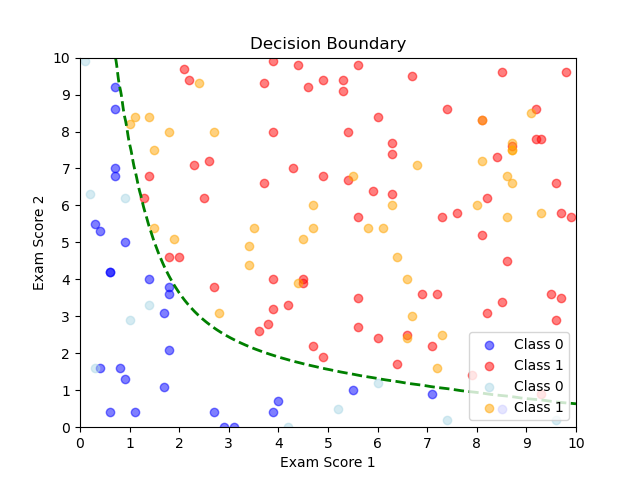
\includegraphics[width=0.9\linewidth]{logistic_regression_result_d=2.png}

\subsection*{plot for $d = 3$}
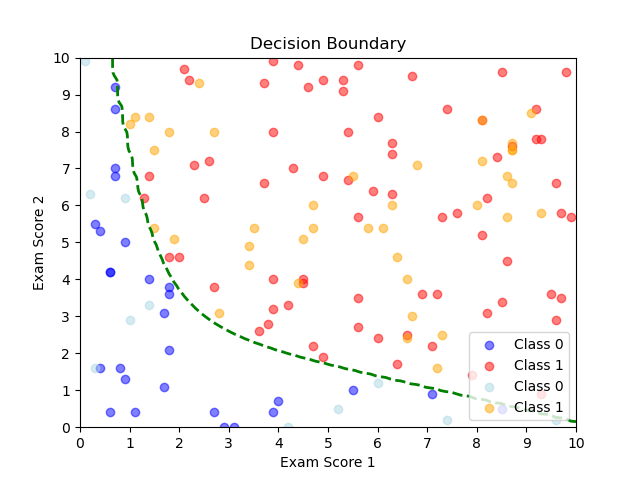
\includegraphics[width=0.9\linewidth]{logistic_regression_result_d=3.png}

\end{document}